\documentclass{article}
\renewcommand \thesection{\roman{section}}
\usepackage[utf8]{inputenc}
\usepackage{mathtools}
\usepackage{amsmath}
\usepackage{amsfonts}
\usepackage{amssymb}
\usepackage{graphicx}
\usepackage[margin=1in]{geometry}
\usepackage{multicol}
\usepackage{enumitem}
\setlist{nolistsep}
\setlength{\columnsep}{1cm}
\title{AP Physics Notes}
\author{Prathmesh Desai}
\date{May 2014}
\begin{document}
\maketitle
\tableofcontents
\newpage
\section{Kinematics}
	\subsection{Position, Velocity, and Acceleration}
    	\begin{multicols}{2}
    		\[
            	\frac{d\vec{x}}{dt}=\vec{v}(t)
            \]
    		\[
            	\frac{d^2\vec{x}}{dt^2}=\frac{d\vec{v}}{dt}=\vec{a}(t)
            \]
    		\[
            	\bar{v}=\frac{\Delta{x}}{\Delta{t}}
            \]
    		\[
            	\bar{a}=\frac{\Delta{v}}{\Delta{t}}
            \]
    		\[
            	\vec{v_f}=\vec{v_i}+\vec{a}t
            \]
    		\[
            	\vec{d}=\vec{v_i}t+\frac{1}{2}\vec{a}t^2
            \]
    		\[
            	\vec{v_f}^2=\vec{v_i}^2+2\vec{a}(\Delta{x})
            \]
    		\[
            	g=-9.8\frac{m}{s^2}
            \]
    
    		\columnbreak
    
    		Freefall and Projectile Motion:
    		\vspace{3mm}
    		\begin{itemize}
    			\item All free-falling objects do not encounter air resistance\ldots in an ideal world
    			\item All free-falling objects (on Earth) accelerate downwards at a rate of approximately $9.8\frac{m}{s^2}$
    			\item All free-falling objects have a constant $v_x$
    			\item $v_y=0$ \ldots at maximum of y-value of projectile
    		\end{itemize}
    
    		\vspace{2ex}
    		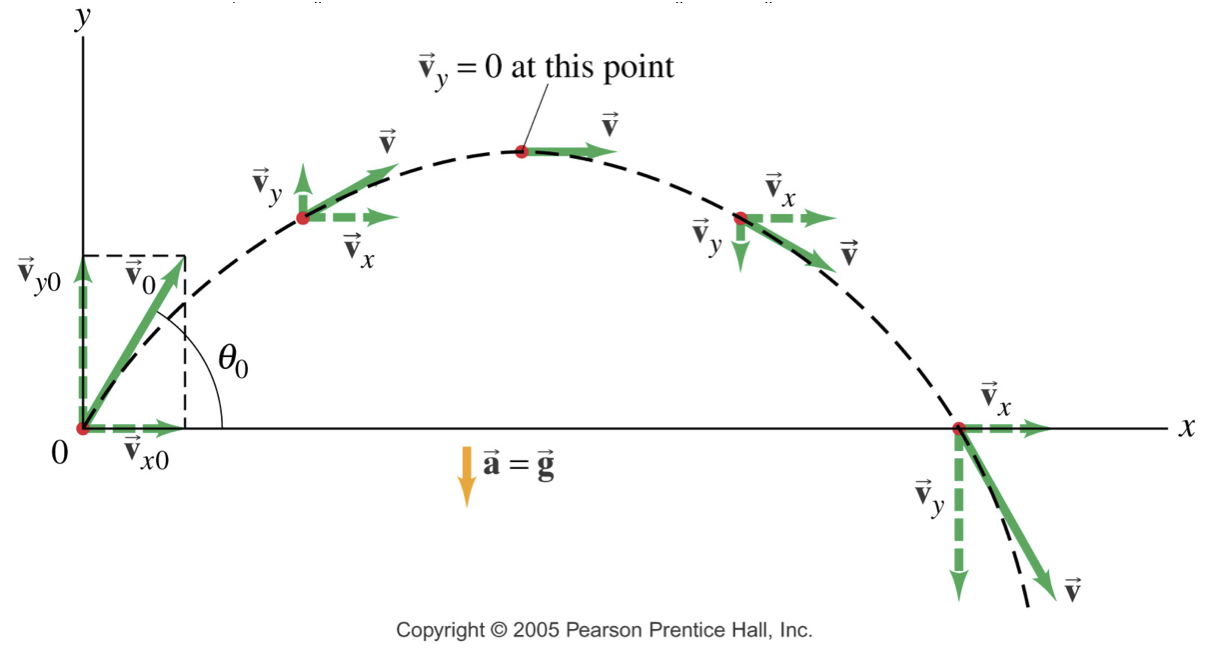
\includegraphics[width=8cm]{ProjectileMotion.jpg}
    	\end{multicols}
    \noindent\textbf{Sample Problems:}
    	\begin{multicols}{2}
    		A loose nail falls from the top of an elevator shaft.  At the same instant 25 m below is the roof of an elevator car rising at a constant 3.0 m/s. \\*\\* Find: \\*
    		\begin{enumerate}[label=\alph*]
    			\item Position \\*
    			\item Velocity of the nail just before it hits the roof of the elevator car\\*
    		\end{enumerate}
    		Nail: $v_i$ = 0$\frac{m}{s}$ and $d_y$ = 25m, above elevator\\*
    		Elevator: $v_i$ = 3$\frac{m}{s}$, up and $d_y$ = 0m
    
    		\columnbreak
    
    		\textit{In time, $t$, the vertical distance travelled equals:}
    		\[
            	\Delta{x_n}=25m-\frac{gt^2}{2} \indent \Delta{x_e}=0m-v_et
            \]
    
    		\textit{So, $t$ is the solution to the equation:}
    		\[
            	25m-\frac{gt^2}{2}=0m-v_et \indent t=1.9733s
            \]
    
    		\begin{enumerate}[label=\alph*]
    			\item $x=v_et=(-3\frac{m}{s})(1.9733s)=19m,$ up \\*
    			\item $v_n=gt=(-9.8\frac{m}{s^2})(1.9733s)=19\frac{m}{s},$ down
    		\end{enumerate}
    
    	\end{multicols}
    
    \noindent\centerline{\rule{5cm}{0.4pt}}
    
    	\begin {multicols}{2}
    		Suppose a volleyball player wants to serve the ball such that it just barely passes over the net.  Let x represent the horizontal distance to the net and y represent the height of the net relative to the launch point of the ball.
    		\\*\\*
    		Derive an equation that gives the initial launch angle in terms of x and y.
    	\columnbreak
    		\[
            	y=v_i\sin(\theta)t+\frac{at^2}{2} \indent x=v_i\cos(\theta)t
            \]
    		\[
            	v_i=\frac{y+\frac{gt^2}{2}}{t\sin(\theta)}=\frac{x}{t\cos(\theta)}
            \]
    		\[
            	y+\frac{gt^2}{2}=\frac{xt\sin(\theta)}{t\cos(\theta)}=xtan(\theta)
            \]
    		\[
            	y=\frac{gt^2}{2} \indent y+y=xtan(\theta) \indent \therefore \theta=tan^{-1}(\frac{2y}{x})
            \]
    	\end{multicols}
        
\section{Dynamics}
  	\subsection{Newton's First Law of Motion}
  
  		Every object in a state of uniform motion tends to remain in that state of motion unless an external force is applied to it.
  		\\\\
  		\textbf{Inertia}: a property of matter by which it continues in its existing state of rest or uniform motion in a straight line, unless that state is changed by an external force.
  
  		\begin{multicols}{2}
  			\textbf{For instance} inertia is evident in the famous ``parlor trick'' where the  tablecloth is pulled from under the plates, tumblers, and silverware in a full dining setting. In this case the objects on the table are at rest, and, unless an external force is applied to each individual object, they will remain at rest. When the table cloth is pulled out from under the objects there are no significant external forces in play (friction is negligible if done correctly), and as a result only the tablecloth is removed.
  		\columnbreak
  			\centerline{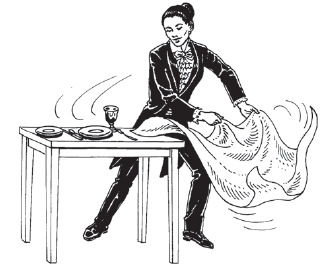
\includegraphics[width=5cm]{tableInertia.png}}
  		\end{multicols}
  
  	\subsection{Newton's Second Law of Motion}
  
  		The vector sum of the forces $\vec{F}$ on an object is equal to the mass $m$ of that object multiplied by the acceleration $\vec{a}$ of the object. $\vec{a}$ and $m$ are both directly proportional to $\vec{F}$. The $\vec{F}$ is the vector sum of all \emph{EXTERNAL} forces, so any internal interactions can be ignored.
  
  		\[
        	\Sigma\vec{F}=m\vec{a}
        \]
  
  	\subsection{Newton's Third Law of Motion}
  
  		When one body exerts a force on a second body, the second body simultaneously exerts a force equal in magnitude and opposite in direction on the first body.
  		\begin{multicols}{2}
  			\centerline{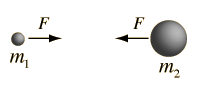
\includegraphics[width=6cm]{thirdLaw.png}}
  		\columnbreak
  			Without specifying the nature or origin of the forces on the two masses, Newton's 3rd law states that if they arise from the two masses themselves, they must be equal in magnitude but opposite in direction so that no net force arises from purely internal forces.
  		\end{multicols}
  
  	\subsection{Frictional Forces}
  
  		The weight of an object is defined as the force of gravity on the object and may be calculated as the mass times the acceleration of gravity.
  		\[
        	Weight=F_g=mg \indent g=9.8\frac{m}{s^2}
        \]
  
  		Frictional resistance to the relative motion of two solid objects is usually proportional to the force which presses the surfaces together as well as the roughness of the surfaces. Since it is the force perpendicular or ``normal'' to the surfaces which affects the frictional resistance, this force is typically called the ``normal force'' and designated by $F_N$.
  		\[
        	F_{friction}=\mu F_N
        \]
  		\begin{multicols}{2}
  			\noindent$F_N$ is the component of force perpendicular to the surface (surface being a plane) of contact.
  			\[
            	\mu_s>\mu_k
            \]
  			\centerline{$\mu_s$ -- Coefficient of static friction}\\*
  			\centerline{$\mu_k$ -- Coefficient of kinetic friction}
  		\columnbreak
  			\centerline{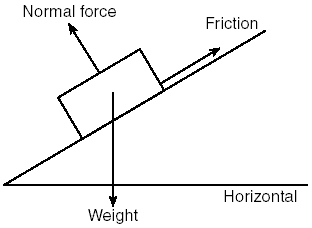
\includegraphics[width=4cm]{normalForce.png}}
  		\end{multicols}
  
  	\subsection{Atwood's Machine}
  		Frictionless and massless pulley:
  
  		\begin{multicols}{2}
  			\centerline{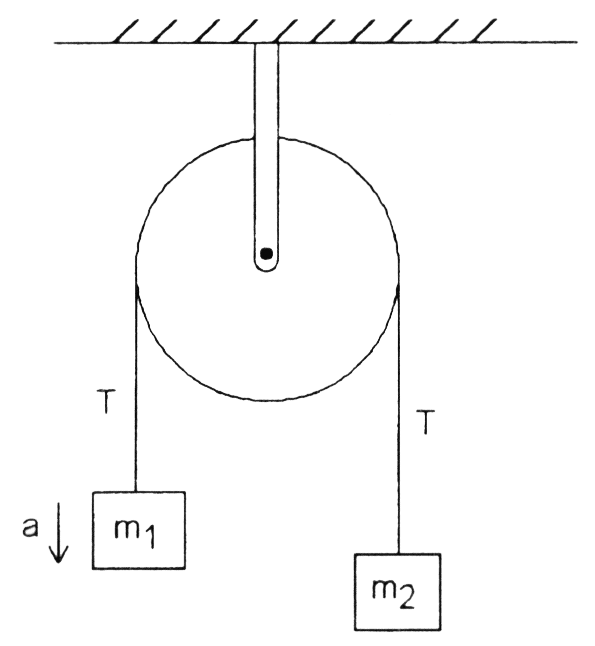
\includegraphics[width=3cm]{atwood.png}}
  		\columnbreak
        	\[
            	m_2>m_1
            \]
  			\[
            	T=m_1g+\Sigma\vec{F}=m_1g+m_1\vec{a}=m_2g-m_2\vec{a}
            \]
  			\[
            	m_2g-m_1g-m_1\vec{a}=m_2\vec{a}
            \]
  			\[
            	\therefore\vec{a}=\frac{g(m_2-m_1)}{m_2+m_1}
            \]
  		\end{multicols}
  
  	\subsection{Air Resistance}
  		\textbf{Air resistance} is the result of collisions of the object's leading surface with air molecules, and it depends on the speed of the object and the cross-sectional area of the object. Eventually the force of air resistance equals the force of gravity, and prohibits any futher acceleration ($\vec{F_{net}}=0$). This state of freefall is called \textbf{terminal velocity}. Usually it is assumed that air resistance is proportional to speed or that it is proportional to the square of the speed (more accurate).
  		\[
        	\vec{F}_{D}\approx -k\vec{v} \indent or \indent \vec{F}_{D}\approx k\vec{v}^2
            \indent \text{Force of drag through a fluid: } \frac{1}{2}\rho v^2 C_D A
        \]
        Air Resistance is demonstrated in the following Position, Velocity, and Acceleration vs. Time graphs:\\
        \centerline{
  			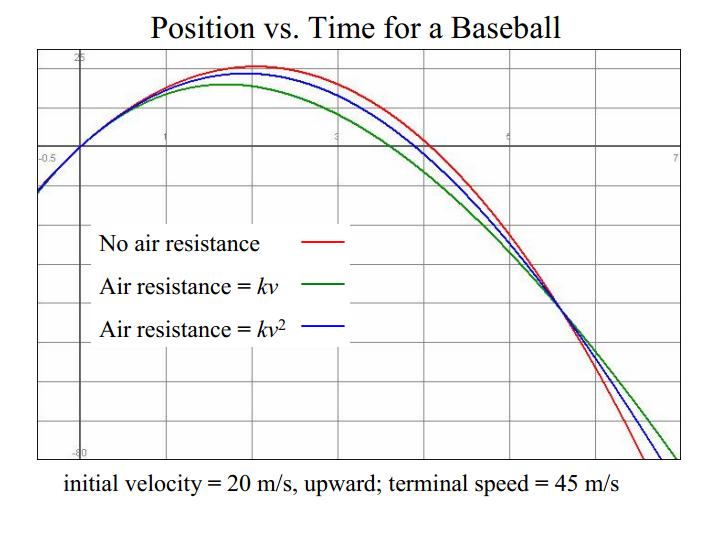
\includegraphics[width=5cm]{pvt_air.png}
        	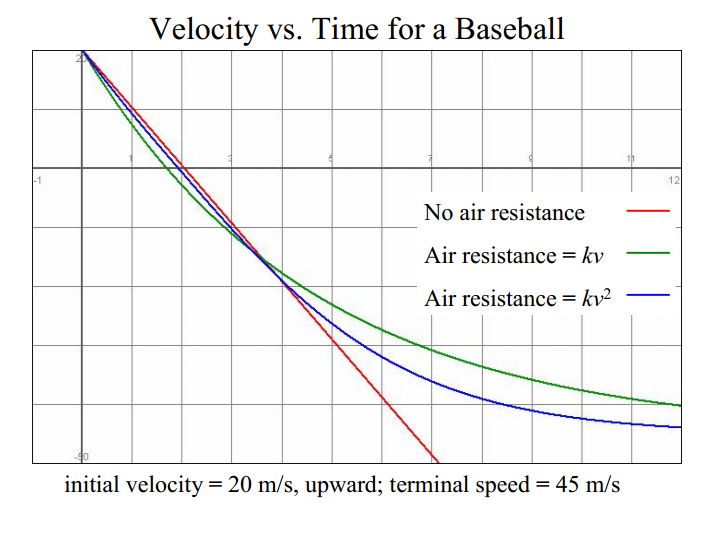
\includegraphics[width=5cm]{vvt_air.png}
        	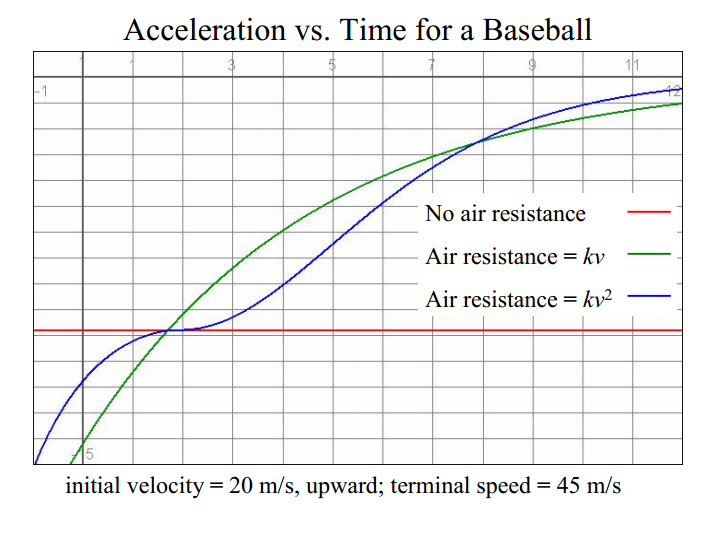
\includegraphics[width=5cm]{avt_air.png}
        }
  		\textbf{Sample Problems:}
        \begin{multicols}{2}
        Suppose a baseball of mass $m$ is falling through the air at a velocity $\vec{v}$ that is proportional to drag force $\vec{F}_D$. Solve for $\vec{v}(t)$.
        \[
        	\Sigma\vec{F}=m\vec{a}=\vec{F}_g-\vec{F}_D=mg-k\vec{v}
        \]
        Guess and check method:
        \[
        	\vec{v}(t)=Ae^{Bt}+C \indent \vec{a}=\frac{d\vec{v}}{dt}=ABe^{Bt}
        \]
        \[
        	m\vec{a}=mg-k\vec{v} \indent m(ABe^{Bt})=mg-k(Ae^{Bt}+C)
        \]
        \[
        	mABe^{Bt}=mg-kAe^{Bt}-kC
        \]
        \columnbreak
        \[
        	0=mg-kC \indent mg=kC \indent C=\frac{mg}{k} \indent \text{(C)}
        \]
        \[
        	mABe^{Bt}=-kAe^{Bt} \indent mB=-k \indent B=\frac{-k}{m} \indent \text{(B)}
        \]
        \[
        	\vec{v}(t)=Ae^{Bt}+C=Ae^{\frac{-kt}{m}}+\frac{mg}{k}
        \]
        \[
        	\vec{v}(0)=Ae^{-k(0)}{m}+\frac{mg}{k} \indent A=\frac{-mg}{k} \indent \text{(A)}
        \]
        \[
        	\therefore \indent \vec{v}(t)=\frac{mg}{k}(1-e^{\frac{-kt}{m}})
        \]
        \end{multicols}
        
        \noindent\centerline{\rule{5cm}{0.4pt}}
  		
        \begin{multicols}{2}
  			Must an object always move in the direction of the net force acting upon it?  Explain and give examples to support your answer.
  			\vfill
  		\columnbreak
  			\textit{No, an object doesn't necessarily have to move in the direction of the $\vec{F}_{net}$. An example is circular motion, where the $\vec{F}_{net}$ is towards the center.}
  		\end{multicols}
  
  		\noindent\centerline{\rule{5cm}{0.4pt}}
  
  		\begin{multicols}{2}
  			A cart on wheels is loaded with books.  In order to move the cart you must exert a relatively great force to start it moving but then a much smaller force to keep it moving.  Use Newton’s laws to explain.
  			\vfill
  		\columnbreak
  			\textit{An object at rest has the tendency to remain at rest, and so the cart loaded with books (when at rest) wants to remain in it's state of rest. Thus, in order to move it one must exert a greater force than the force required to keep the cart in motion.}
  		\end{multicols}
  
  		\noindent\centerline{\rule{5cm}{0.4pt}}
  
  		\begin{multicols}{2}
  			A pair of fuzzy dice hangs from the ceiling of a car that accelerates forward at $3.00\frac{m}{s^2}$.  Assuming the dice have the same acceleration as the car, what is the angle $\theta$ as shown in the diagram below?\\\\
  			\centerline{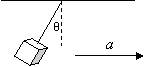
\includegraphics[width=5cm]{dice.png}}
  		\columnbreak
  			\[
            	\Sigma\vec{F}=m\vec{a}=\vec{T}\sin(\theta)
            \]
  			\[
            	\vec{T}\cos(\theta)=mg \indent \vec{T}=\frac{mg}{\cos(\theta)}
            \]
  			\[
            	m\vec{a}=\frac{mg\sin(\theta)}{\cos(\theta)}
            \]
  			\[
            	\frac{\vec{a}}{g}=tan(\theta)
            \]
  			\[
            	\therefore\theta=tan^{-1}\frac{\vec{a}}{g}=tan^{-1}(\frac{3.00\frac{m}{s^2}}{9.8\frac{m}{s^2}})=17.02^{\circ}
            \]
  		\end{multicols}
  
  		\noindent\centerline{\rule{5cm}{0.4pt}}
  
  		\begin{multicols}{2}
  			As shown in the diagram below, two blocks are connected by a lightweight cord that passes over a frictionless, massless pulley.  The bottom block has a mass of $2.00 kg$ and the top block has mass $0.500 kg$.  The coefficient of kinetic friction at each sliding surface is equal to $0.10$.  The two blocks are release from rest.  Determine the acceleration, $\vec{a}$, of each block.\\\\
            \vfill
  			\centerline{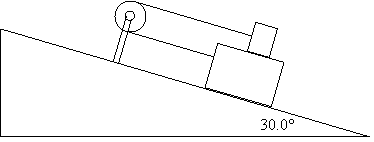
\includegraphics[width=6cm]{frictionPlane.png}}
  			\vfill
  		\columnbreak
  			\noindent\textit{Net force for $m_1$ (smaller block):}
  			\[
            	\Sigma\vec{F}=m_1\vec{a}=T-m_1 g\sin(\theta)-\mu_km_1g\cos(\theta)
            \]
  			\textit{Net force for $m_2$ (larger block):}
  			\[
            	\Sigma\vec{F}=m_2\vec{a}=m_2g\sin(\theta)-T-\mu_km_1g\cos(\theta)-\mu_k(m_1+m_2)g\cos(\theta)
            \]
            \textit{Solve for $\vec{a}$:}
            \[
            	\vec{T}=m_2g\sin(\theta)-\mu_km_1g\cos(\theta)-\mu_k(m_1+m_2)g\cos(\theta)-m_2\vec{a}
            \]
            \[
            	T=m_1\vec{a}+m_1 g\sin(\theta)+\mu_km_1g\cos(\theta)
            \]
            \[
            	\vec{a}=\frac
                {-g((3m_1+m_2)\cos(\theta)\mu_k+(m_1-m_2)\sin(\theta))}
                {(m_1+m_2)}
            \]
            \[
            	\therefore\text{Small Block: }\vec{a}=1.75\frac{m}{s^2} \text{, $150^{\circ}$}
            \]
            \[
            	\therefore\text{Large Block: }\vec{a}=1.75\frac{m}{s^2} \text{, $330^{\circ}$}
            \]
       	\end{multicols}
          
\section{Circular Motion and Gravity}
  
  	\subsection{Uniform Circular Motion}
  		Anything in circular motion is always accelerating towards the center, this value is called centripetal acceleration. Centripetal means ``center-seeking''. Velocity in circular motion is directed tangential to the circular path of the object.
  		\begin{multicols}{2}
        	\centerline{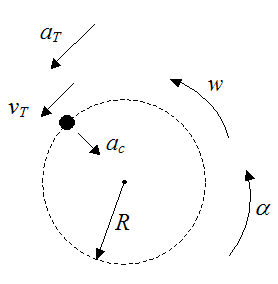
\includegraphics[width=5cm]{circularMotion.png}}
            \columnbreak
  			\[
            	\vec{v}=\frac{2\pi r}{T}
            \]
  			\[
            	\vec{a_c}=\frac{v^2}{r}
            \]
  			\[
            	\Sigma\vec{F}=m(\vec{a_c})=\frac{mv^2}{r}
            \]
            \[
            	f=\frac{1}{T}
            \]
      	\end{multicols}
        
		\textbf{Sample Problem:}
        \begin{multicols}{2}
            A car of mass $m$ goes around a curve of radius $r$ banked at an angle of $\theta$ above horizontal. (a) At what speed could the car complete this curve without the aid of lateral friction? (b) Given $\mu_s$ determine the maximum speed at which the car can go around the same curve.
            \centerline{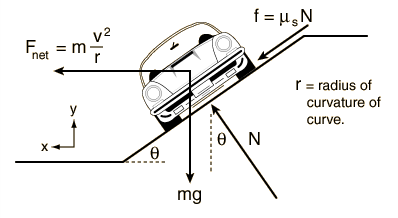
\includegraphics[width=5cm]{bankedCurve.png}}
            Because $\Sigma\vec{F}$ is only in the x-direction we do not need to worry about the y-component.
            \[
            	mg=N\cos(\theta)
            \]
            \[
            	N=\frac{mg}{cos(\theta)}
            \]
            \[
            	N_x=N\sin(\theta)=mg\tan(\theta)
            \]
            \[
            	-N=\Sigma\vec{F}=\frac{-mv^2}{r}
            \]
            \[
            	g\tan(\theta)=\frac{v^2}{r}
            \]
            \[
            	\therefore \vec{v}=\sqrt{rg\tan(\theta)}
            \]
            \vfill
		\columnbreak
            \noindent{y-direction ($\Sigma\vec{F}=0$):}
            \[
            	N\cos(\theta)-mg-f\sin(\theta)=0
            \]
            \[
            	N\cos(\theta)-\mu_sN\sin(\theta)=mg
            \]
            \[
            	N=\frac{mg}{\cos(\theta)-\mu_s\sin(\theta)}
            \]
            x-direction($\Sigma\vec{F}=\frac{mv^2}{r}$)
            \[
            	-f\cos(\theta)-N\sin(\theta)=-\frac{mv^2}{r}
			\]
            \[
            	N(\sin(\theta)+\mu_s\cos(\theta))=\frac{mv^2}{r}
            \]
            \[
            	N=\frac{mv^2}{r(\sin(\theta)+\mu_s\cos(\theta))}
            \]
            Solve for $\vec{v}$:
            \[
            	N=\frac{mg}{\cos(\theta)-\mu_s\sin(\theta)}=\frac{mv^2}{r(\sin(\theta)+\mu_s\cos(\theta))}
            \]
            \[
            	\therefore \vec{v}=\sqrt{rg(\frac{\sin(\theta)+\mu_s\cos(\theta)}{\cos(\theta)-\mu_s\sin(\theta)})}
            \]
        \end{multicols}
        
	\subsection{Parametric Equations}
    	When a situation is two- or three-dimensional (which is essintially all the time), the position/velocity/acceleration can be determined using parametric equations. Parametric equations are basically equations (shocker!) that describe the behaviour of the components of the object, rather than the vector sum of the components.
        \[
        	r_x=x(t) \hspace{1ex} \hat{i} \indent
            r_y=y(t) \hspace{1ex} \hat{j} \indent
            r_z=z(t) \hspace{1ex} \hat{k} \indent
        \]
        \[
        	v_x=\frac{dx}{dt} \hspace{1ex} \hat{i} \indent
            v_y=\frac{dy}{dt} \hspace{1ex} \hat{j} \indent
            v_z=\frac{dz}{dt} \hspace{1ex} \hat{k}
        \]
        \[
        	a_x=\frac{dv_x}{dt}=\frac{d^2v_x}{dt^2} \hspace{1ex} \hat{i} \indent
            a_y=\frac{dv_y}{dt}=\frac{d^2v_y}{dt^2} \hspace{1ex} \hat{j} \indent
            a_z=\frac{dv_z}{dt}=\frac{d^2v_z}{dt^2} \hspace{1ex} \hat{k}
        \]
        \[
        	\vec{r}^2=r_x^2+r_y^2+r_z^2
        \]
        \[
        	\vec{v}^2=v_x^2+v_y^2+v_z^2
        \]
        \[
        	\vec{a}^2=a_x^2+a_y^2+a_z^2
        \]

  	\subsection{Non-uniform Circular Motion}
    	Non-uniform circular motion is any case in which an object moving in a circular path has a varying speed. The tangential acceleration is non-zero; the speed is changing.The net acceleration is no longer pointing towards the center, so there are two components of acceleration that we would need to account for:\vspace{1ex}
        \begin{multicols}{2}
            \centerline{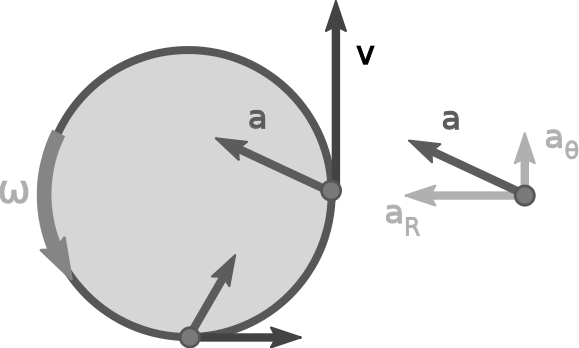
\includegraphics[width=6cm]{noncirc.png}}
       	\columnbreak
        	\begin{enumerate}
        		\item Radial/centripetal acceleration ($a_R$)
            	\item Tangential acceleration ($a_\theta$)
        	\end{enumerate}
        	\[
            	\lvert\vec{a}\rvert=\sqrt{\vec{a_\theta}^2+\vec{a_R}^2}
            \]
            We note that velocity, tangential acceleration and tangential force all act along the same direction.
            \[
            	a_\theta=\frac{dv}{dt}
            \]
        \end{multicols}
        
        \noindent\textbf{Sample Problem:}
        \begin{multicols}{2}
        A kid plays with a yo-yo of mass $m$ and twirls it in a vertical circle.  The length of the string is $l$.  The kid twirls it just fast enough to keep it moving in a complete circle – this results in a centripetal acceleration of 5.00 $g$ at the lowest point. (a) Find the speed of the yo-yo at the highest point. (b) Find the speed at the lowest point.
        \vfill
        \columnbreak
        \noindent{\textit{Find $v$ at highest point:}}
        \[
        	\Sigma\vec{F}=m\vec{a}=mg \indent
            \vec{a}=g
        \]
        \[
        	\vec{a}=\frac{v^2}{r} \indent
            v=\sqrt{\vec{a}r}=\sqrt{gr}
        \]
        \textit{Find $v$ at lowest point:}
        \[
        	\vec{a}=5g \indent
            v=\sqrt{\vec{a}r}=\sqrt{5gr}
        \]        
        \end{multicols}

	\subsection{Newton's Universal Law of Gravitation}
    	Newton's law of universal gravitation states that any two bodies in the universe attract each other with a force that is directly proportional to the product of their masses and inversely proportional to the square of the distance between them.
        
        \[
        	\vec{F_G}=G\frac{m_1m_2}{r^2} \indent
            G=6.674x10^{-11}\frac{Nm^2}{kg^2}
        \]
        
	\subsection{Gravitational Field Strenth}
    	A value ($g$) that is the strength of the gravitational field (acceleration due to gravity) at some place given mass $M$ and radius $r^2$ of object producing the field.
        \[
        	g=\frac{GM}{r^2}
        \]
        
  		\noindent\textbf{Sample Problems:}
        
        \begin{multicols}{2}
        	In 1995, the Galileo robotic spacecraft released a probe into Jupiter’s atmosphere.  When traveling at $v_1 \frac{m}{s}$ the $m$ kg-probe’s main chute deployed and slowed it to $v_2 \frac{m}{s}$ in $t$ seconds.\\\\ (a) Find the force of Jupiter’s gravity acting on the probe.\\\\ (b) Determine the force that the cords of the chute had to withstand.
		\columnbreak
        \vfill
        	\noindent{Solve for $F_{jupiter}$}
        	\[
            	F_{jupiter}=G\frac{m_{chute}m_{jupiter}}{r_{jupiter}^2}
            \]
            Solve for $F_T$ exerted by the cords:
            \[
            	\Sigma\vec{F}=m\vec{a}=F_T-F_g
            \]
            \[
            	m(\frac{\Delta v}{t})=F_T-F_g
            \]
            \[
            	F_T=G\frac{m_{chute}m_{jupiter}}{r_{jupiter}^2}+\frac{v_1-v_2}{t}
            \]
        \end{multicols}
        
        \noindent{\centerline{\rule{5cm}{0.4pt}}}
        
        \begin{multicols}{2}
        	It can be shown that the value of $g$ inside an empty spherical shell is zero at all points inside the shell (no matter how massive the shell).  Suppose the Earth had uniform density.\\\\ (a) Use these two ideas to solve for $g$ inside the Earth. (Inside the Earth, at any point a distance $r$ from the center, only the mass contained in a sphere of radius $r$ has a net gravitational effect.  All mass between $r$ and the surface has a net gravitational effect of zero.)\\\\ (b) Sketch a graph of $g$ versus $r$ extending from $r = 0$ to $r = 2R_E$.\\\\            \centerline{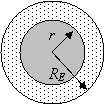
\includegraphics[width=6cm]{p27.png}}
            \vfill
		\columnbreak
        	\noindent{Write down equations:}
            \[
            	F_g=G\frac{m_1m_2}{r^2} \indent
                g=\frac{GM_E}{r^2}
            \]
            Find ratio of r and $R_E$
            \[
            	V_r=\frac{4}{3}\pi r^3 \indent
                V_{R_E}=\frac{4}{3}\pi R_E^3
            \]
            \[
            	\frac
                {\frac{4}{3}\pi r^3}
                {\frac{4}{3}\pi R_E^3}
                \indent
                \rightarrow
                \indent
                (\frac{r}{R_E})^3
            \]
            \[
            	g=\frac{GM_Er^3}{r^2R_E^3}=\frac{GM_Er}{R_E^3}
            \]
            \[
            	g=\frac{r}{R_E}g_{surface}
            \]
            Graph $g$ vs. $r$ from $0$ to $2R_E$\\\\
            \centerline{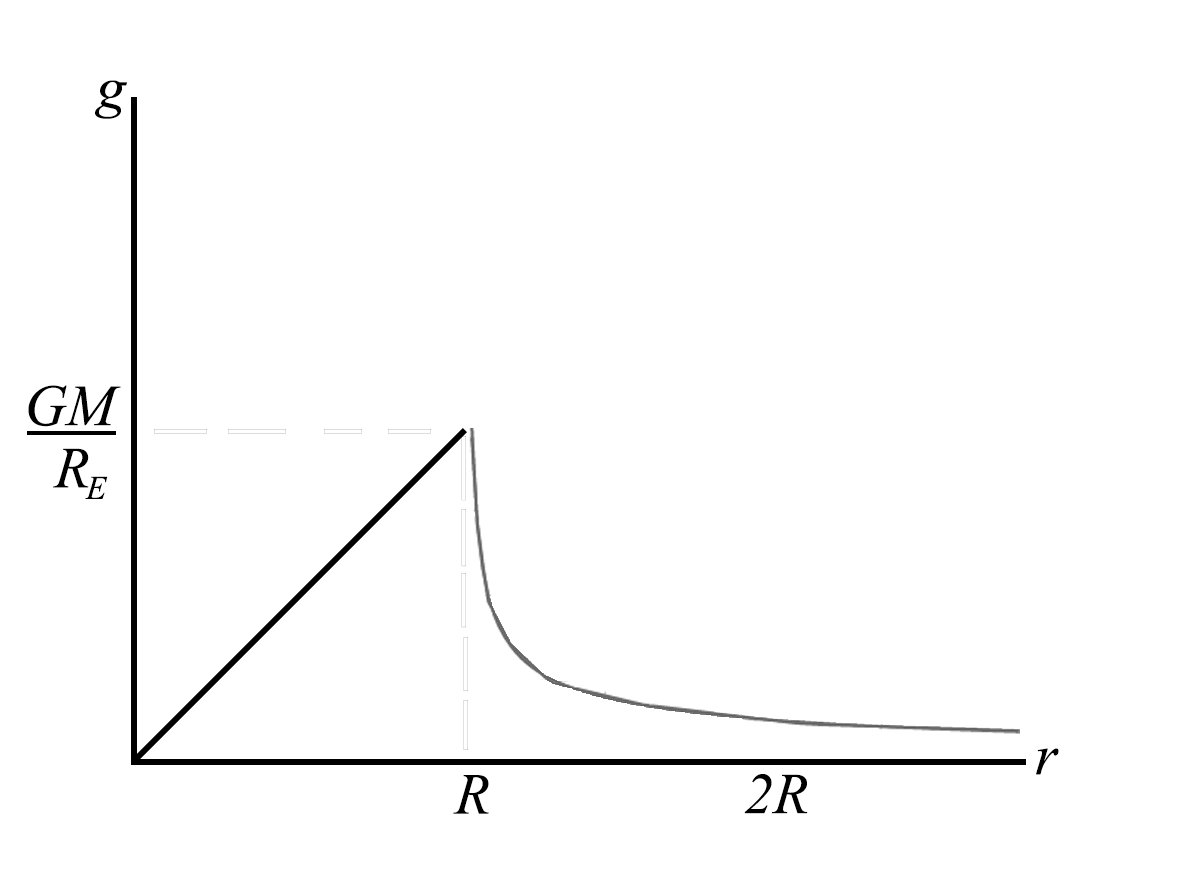
\includegraphics[width=8cm]{graph27.png}}
        \end{multicols}
        
	\subsection{Keplar's Laws of Planetary Motion}
        In astronomy, Kepler's laws of planetary motion are three scientific laws describing the motion of planets around the Sun.
        \vspace{1ex}
        \begin{enumerate}
        	\item The orbit of a planet is an ellipse with the Sun at one of the two foci.
            \item A line segment joining a planet and the Sun sweeps out equal areas during equal intervals of time.
            \item The square of the orbital period of a planet is proportional to the cube of the semi-major axis of its orbit.
        \end{enumerate}
        \begin{multicols}{2}
        	\centerline{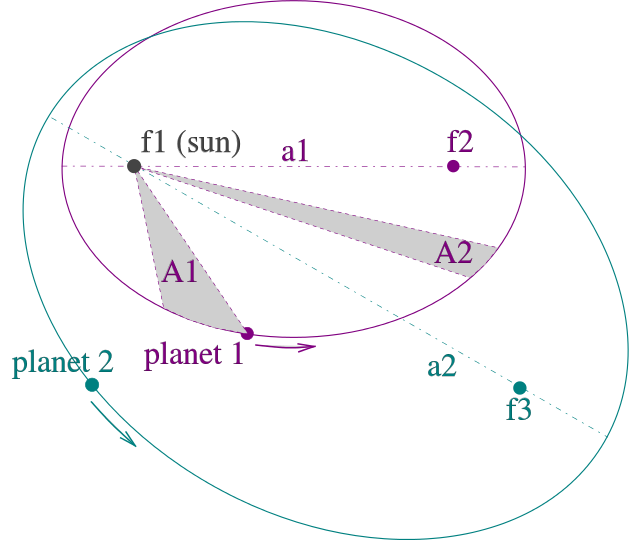
\includegraphics[width=7cm]{keplar.png}}
		\columnbreak
        	Keplar's second law is demonstrated by the image, where $A1=A2$ IF they were both swept out in the same amount of time.
            \\\\
            Derive Keplar's Third Law:
            \[
            	\vec{F}_c=\vec{F}_g \indent
                \frac{m_2\vec{v}^2}{r}=G\frac{m_1m_2}{r^2}
            \]
            \[
            	\vec{v}=\sqrt{\frac{GM}{r}}=\frac{2\pi r}{T}
            \]
            \[
            	\frac{r^3}{T^2}=\frac{GM}{4\pi^2} = constant
            \]
            \[
            	r^3 \propto T^2
            \]
        \end{multicols}
        
        \noindent{\textbf{Sample Problem:}}
        \begin{multicols}{2}
        	
			Two planets travel in circular orbits around a star.  Planet A has speed $v$ and planet B has speed $3v$.\\\\ (a) Find the ratio of the two planets’ orbital radii.\\\\ (b) Find the ratio of the two planets’ periods.
			\vfill
			\columnbreak
			\noindent{Find ratio of orbital radii:}
			\[
				\frac
                {F_A=\frac{Gm_pm_s}{r_A^2}}
                {F_B=\frac{Gm_pm_s}{r_B^2}}
                \indent
                \frac{r_A}{r_B}=\frac
                {3^2}
                {1^2}
			\]
			\[
             	\frac{r_A}{r_B}=9
			\]
			Find ratio of periods:
			\[
             	\frac
                {T_A^2=r_A^3}
                {T_B^2=r_B^3}
                \indent
                \frac
                {T_A}
				{T_B} = \frac{3^3}{1^3}
			\]
			\[
             	\frac{T_A}{T_B}=27
			\]
		\end{multicols}
        
\section{Work and Energy}
        
\end{document}